\begin{figure}[h!]
   \centering
   \begin{subfigure}[b]{0.4\textwidth}
      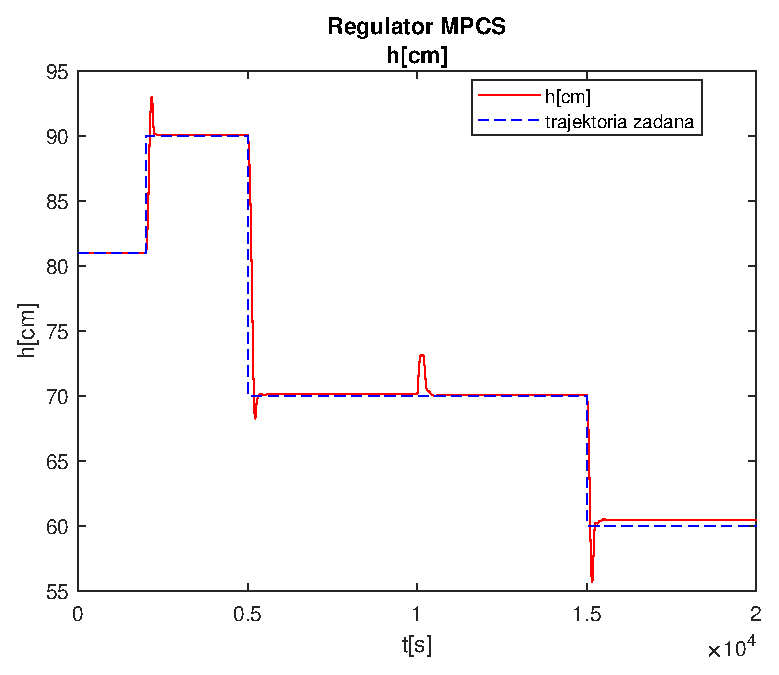
\includegraphics[width=1\linewidth]{img/MPCSanaRK/MPCSRKHN300Nu100l10.eps}
      \caption{}
      \label{fig:fig:MPCSRKN300Nu100l101}
   \end{subfigure}
       
   \begin{subfigure}[b]{0.4\textwidth}
      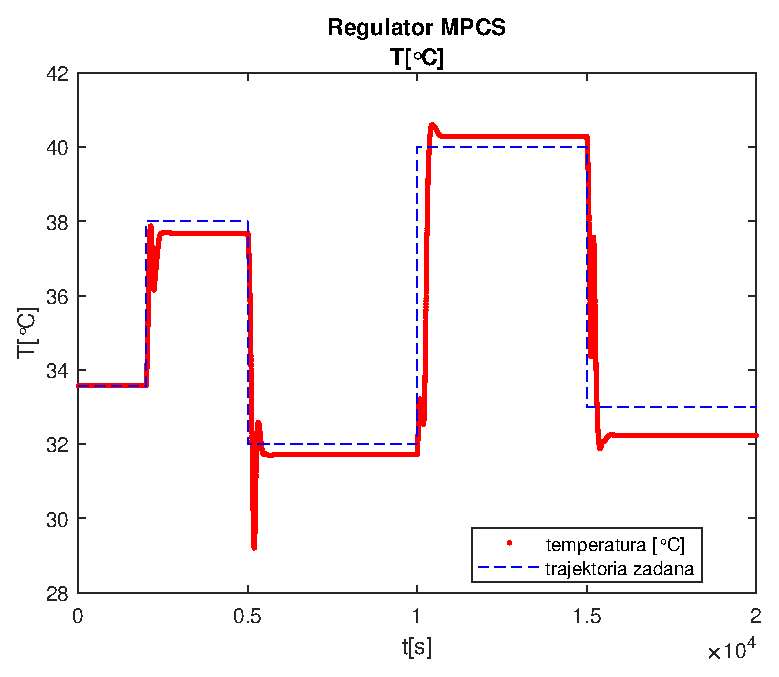
\includegraphics[width=1\linewidth]{img/MPCSanaRK/MPCSRKTN300Nu100l10.eps}
      \caption{}
      \label{fig:fig:MPCSRKN300Nu100l102}
   \end{subfigure}
       
   \begin{subfigure}[b]{0.4\textwidth}
      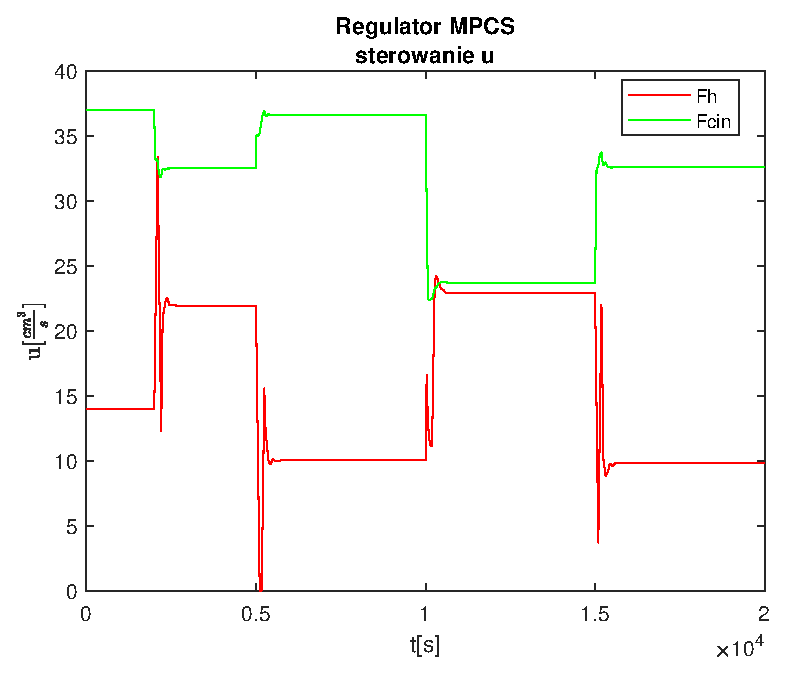
\includegraphics[width=1\linewidth]{img/MPCSanaRK/MPCSRKControlN300Nu100l10.eps}
      \caption{}
      \label{fig:fig:MPCSRKN300Nu100l103}
   \end{subfigure}
       
   \caption{Wykresy dla regulatora MPCS, obiekt nieliniowy, $N = 300$, $N_u = 100$, $\lambda = 0.1$.}
   \label{fig:MPCSRKN300Nu100l10}
\end{figure}
           
